\chapter{Hawkes Process}\label{ch:hawkes}
Chapter \ref{ch:explore} showed that spike onsets cluster. Part of that could just be the time of day and the season. The
question here is whether there is clustering \emph{on top of} that: do spikes trigger more spikes?

\section{The model}
Let $t_1 < t_2 < \dots$ be the spike onset times in hours. A Hawkes process \cite{hawkes1971} has intensity (the instantaneous rate of events)
\begin{equation}
\lambda(t) = \mu(t) + \sum_{t_i < t} n\beta e^{-\beta(t - t_i)},
\end{equation}
where
\begin{itemize}
\item $\mu(t) = \exp(a_{\text{hour}(t)} + b_{\text{month}(t)})$ is the background rate, with one effect per hour of day and one per
month ($b$ of the first month is fixed at 0 so the model is identifiable)
\item every onset adds on average $n$ ``offspring'' onsets, with mean delay $1/\beta$ hours. $n$ is the branching ratio, roughly the
fraction of onsets caused by earlier onsets, and must be below 1 for the process to be stable.
\end{itemize}
$n = 0$ is an inhomogeneous Poisson process, which we fit too, for comparison. The month effect matters: without it, the winter pile
up of spikes would be credited to self-excitation.

\section{Likelihood and fitting}
The log likelihood of a point process \cite{ogata1978} on $[0, T]$ is 
\begin{equation}
\log L = \sum_i \log \lambda(t_i) - \int_0^T \lambda(t)\,dt,
\end{equation}
where the integral of the background is $\sum_{h,m} e^{a_h + b_m} E_{h,m}$, with $E_{h,m}$ the hours the year spends in each
(hour, month) cell, and the integral of the excitation is $n\sum_i(1 - e^{-\beta(T - t_i)})$. Computed directly, the sum inside
$\lambda(t_i)$ runs over all earlier events, which is $O(N^2)$. With an exponential kernel, Ozaki's recursion \cite{ozaki1979}
does it in $O(N)$:
\begin{equation}
R_i = \sum_{j<i} e^{-\beta(t_i - t_j)} = e^{-\beta(t_i - t_{i-1})}(1 + R_{i-1}), \quad R_1 = 0,
\end{equation}
so $\lambda(t_i) = \mu(t_i) + n\beta R_i$. On 20,000 simulated events the recursion matches the direct sum exactly and takes
0.009\,s against 1.4\,s.

We maximise the likelihood with L-BFGS-B over the unconstrained parameters
\[(a_0,\dots,a_{23},\ b_1, \dots, b_{M-1},\ \operatorname{logit} n,\ \log\beta),\]
started from five values of $(n, \beta)$ since the likelihood can have more than one optimum in $\beta$. In some regions, during some hours there are no onsets at
all, in which the optimiser would push the $a_h$ values to $-\infty$ in order to drive the probability $p_{t}^h$ smaller, so we subtract a roughness penalty
\begin{equation}
\frac{\kappa}{2}\sum_{h} (a_h - a_{h+1})^2, \qquad a_{24} = a_0,\ \kappa = 1.
\end{equation}
Reported log likelihoods and AICs are without the penalty.

\section{Model checks}
\textbf{Time rescaling.} If the model is right, the compensator increments $\tau_i = \int_{t_{i-1}}^{t_i}\lambda(t)\,dt$ are
independent Exp(1) \cite{brown2002}, which we test with a Kolmogorov--Smirnov test. 

\section{Results}
Self-excitation wins by a long way everywhere (Table \ref{tab:hawkes}). AIC improves by 40 to 800 over the Poisson model, the Poisson
model fails the time rescaling test badly in every region while the Hawkes model passes in all of them (Figure \ref{fig:rescaling}),
and the observed daily dispersion sits inside the simulated range. The branching ratio is 0.34--0.69: between a third and two
thirds of spike onsets are triggered by an earlier one, with a mean delay of 40 to 90 minutes. The process is sub-critical
everywhere, so clusters die out. This is the motivation for
the decaying spike count features in the forecasting models.

\begin{table}[!htbp]\centering\small
\caption{Hawkes and Poisson fits to spike onsets. $\Delta$AIC is the Poisson AIC minus the Hawkes AIC.}\label{tab:hawkes}
\resizebox{\textwidth}{!}{\begin{tabular}{lrrrrrrrrr}
\toprule
 & onsets & branching\_n & mean\_delay\_min & AIC\_hawkes & AIC\_poisson & dAIC & KS\_p\_hawkes & KS\_p\_poisson & disp\_observed \\
\midrule
NSW1 & 116 & 0.605 & 39.6 & 685 & 959 & 275 & 0.0687 & 1.24e-29 & 4.54 \\
QLD1 & 53 & 0.416 & 42.9 & 428 & 518 & 89.2 & 0.822 & 3.28e-06 & 2.93 \\
SA1 & 309 & 0.689 & 90.3 & 1.73e+03 & 2.53e+03 & 796 & 0.1 & 4.18e-74 & 7.6 \\
TAS1 & 49 & 0.34 & 87.6 & 539 & 580 & 41.1 & 0.864 & 3.46e-06 & 2.34 \\
VIC1 & 49 & 0.604 & 38 & 392 & 553 & 160 & 0.339 & 4.62e-16 & 3.64 \\
\bottomrule
\end{tabular}}
\end{table}

\begin{figure}[!htbp]\centering
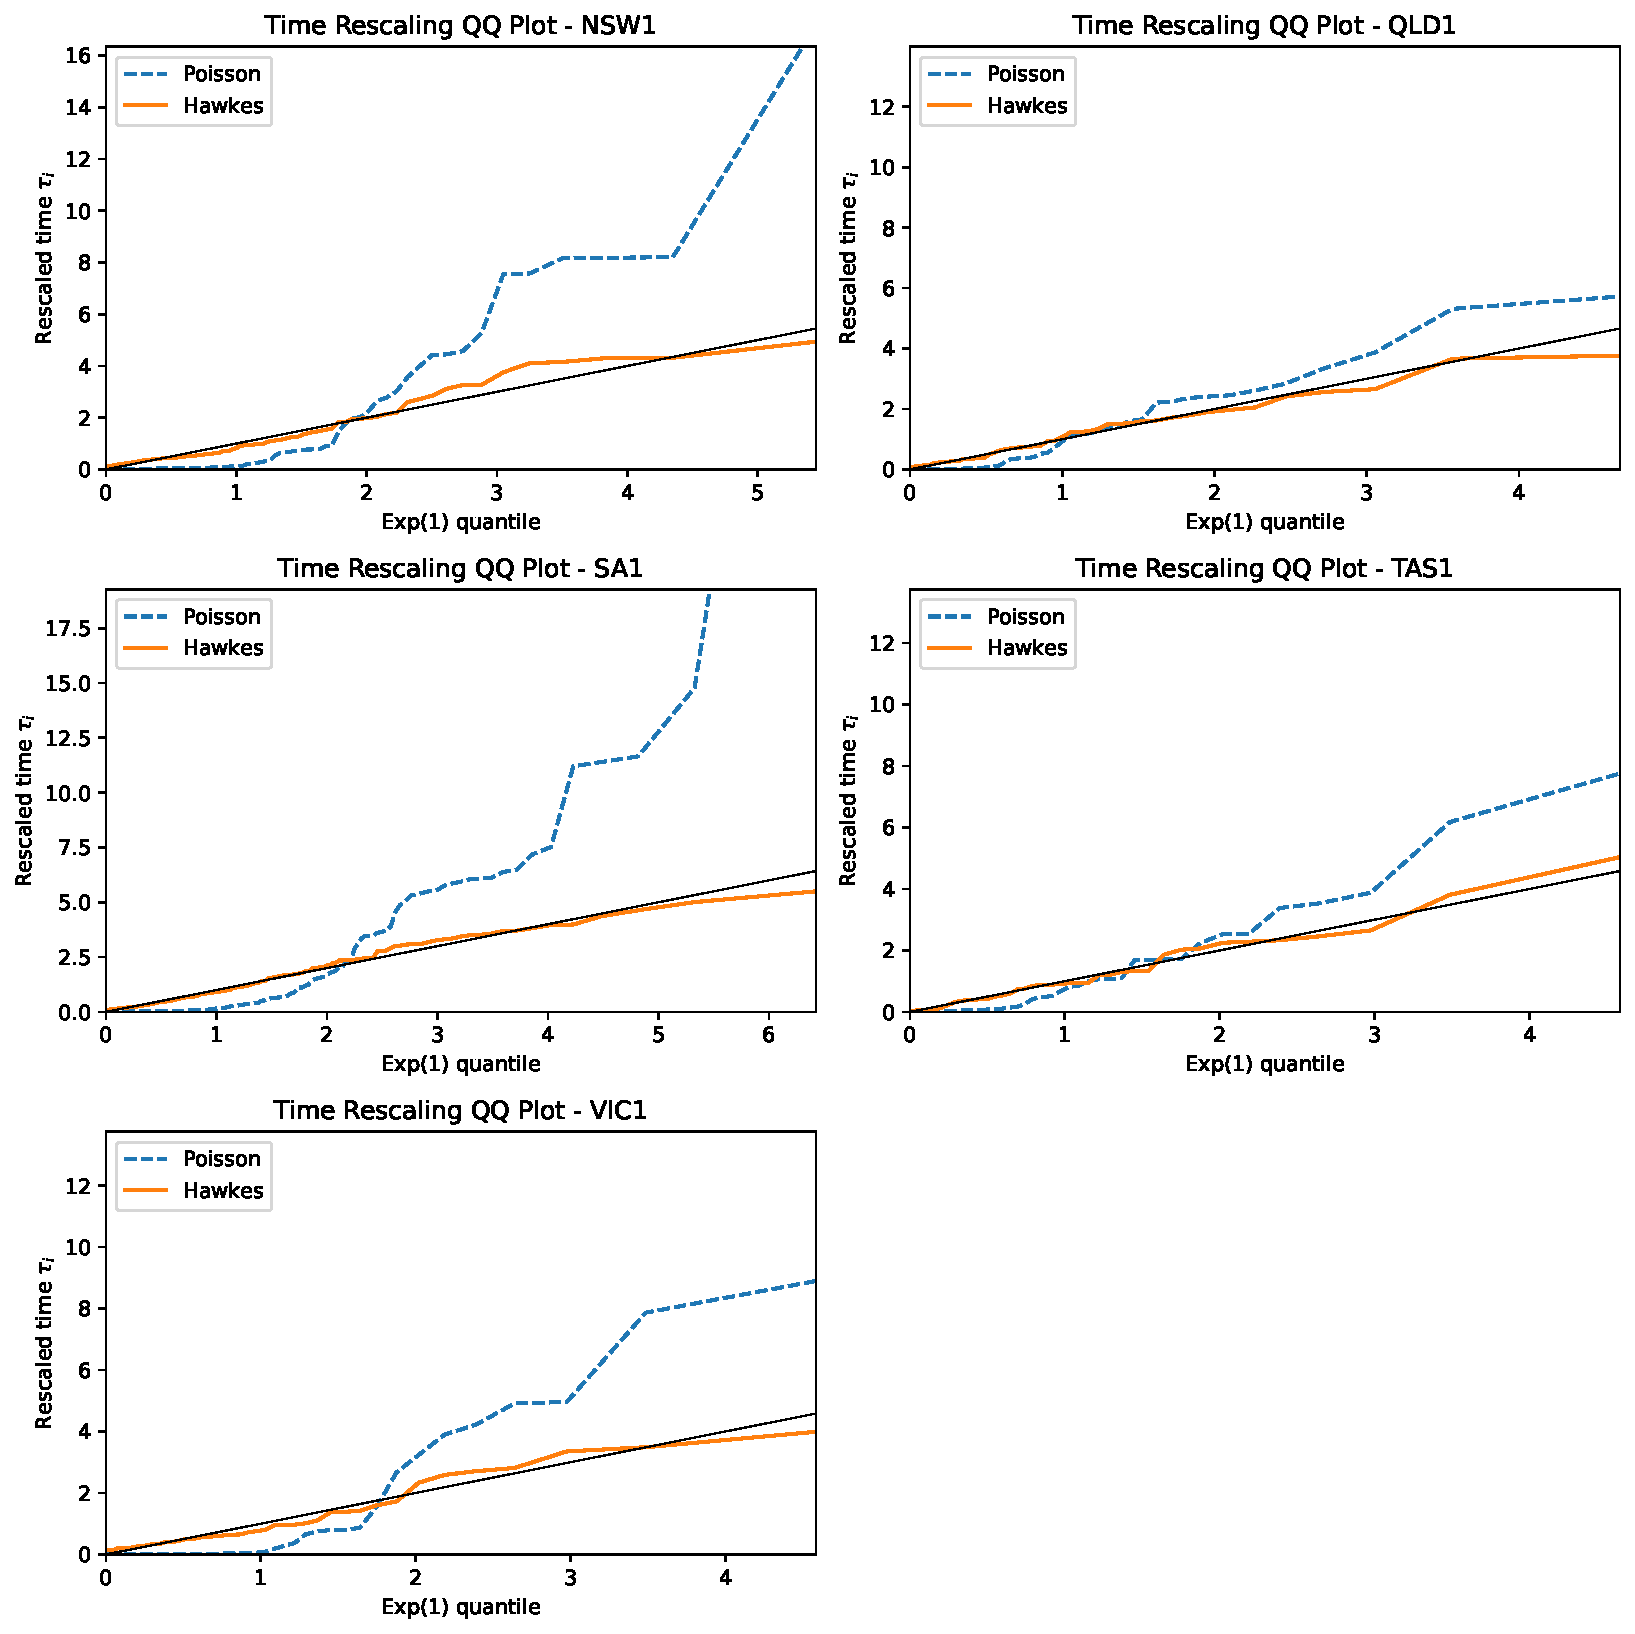
\includegraphics[width=0.8\textwidth]{hawkes_rescaling.pdf}
\caption{Time rescaling QQ plots against Exp(1). Points on the diagonal mean the model accounts for the timing of onsets.}\label{fig:rescaling}
\end{figure}
